\pgfplotsset{compat=1.3, 
wf_axis/.style={
width=9cm,
% xtick={1e-08,1e-07,1e-06,1e-05,0.0001,0.001,0.01},
% xticklabels={\textsf{10\textsuperscript{1}}, 10\textsuperscript{2}, 10\textsuperscript{3}, 10\textsuperscript{4}, 10\textsuperscript{5}, 10\textsuperscript{6}, 10\textsuperscript{7}},
% xmin=1e-8, xmax=1e-2,
font=\sffamily,
ylabel={Yield $\gamma$},
every axis label/.append style={font=\sffamily}
}}

\begin{subfigure}[t]{0.48\textwidth}

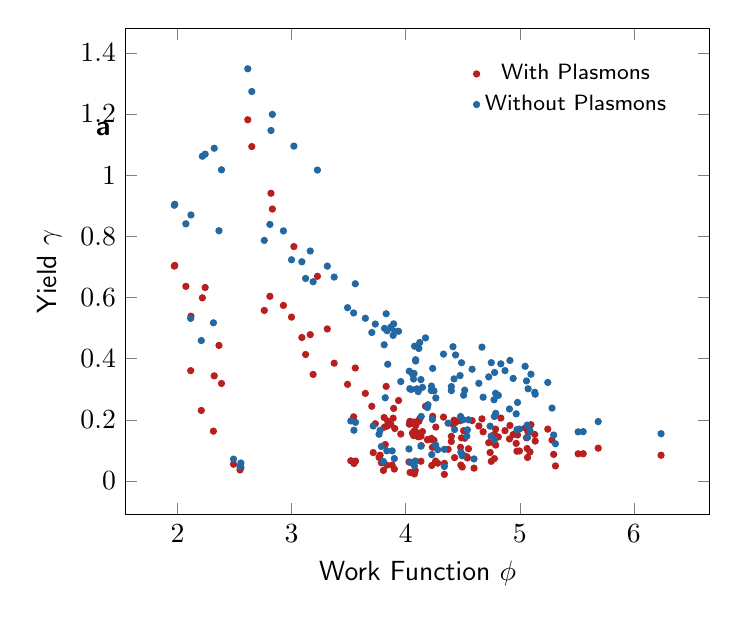
\begin{tikzpicture}[]

\node[anchor=north west, font=\sffamily] at (-0.5, 5.1) {\textbf{a}};

\begin{axis}[
wf_axis,
% height=7cm,
xlabel={Work Function $\phi$},
legend style={
at={(0.95, 0.95)}, anchor=north east, draw=none, font=\footnotesize\sffamily
},
]

% This file was created by tikzplotlib v0.9.1.
\definecolor{color0}{rgb}{0.72156862745098,0.12156862745098,0.12156862745098}
\definecolor{color1}{rgb}{0.137254901960784,0.407843137254902,0.635294117647059}

\addplot [semithick, color0, mark=*, mark size=1, mark options={solid}, only marks]
table {%
4.2339947776178 0.110085644425969
4.13604969014312 0.115493816634617
4.37178442476762 0.10339969200062
4.26366279001154 0.176209403639935
4.03603081275938 0.194701377157733
4.04833302520052 0.192911359851125
4.42826631781476 0.0761869666581625
4.54097859195183 0.0751245806804158
4.75014842130832 0.0640973519205594
5.08945431872201 0.094679824250008
4.97476811855844 0.097274566497049
4.99691000780169 0.0981076433550597
2.32164221855572 0.343733298088694
2.38539824080557 0.318810110274459
2.3145742661612 0.162749004688299
5.31255487263241 0.0490834529142897
4.50285915539127 0.0843347369685517
3.82061880099801 0.119025157277424
4.05899885952132 0.156366323022569
4.0686140341884 0.148447016519934
4.13333249166534 0.146302093517762
2.76044973482305 0.557645529243336
2.80971115145645 0.603914839698665
2.9280118299065 0.574081547837845
3.80466657162114 0.0344522462541396
4.08391155609067 0.0345594178126328
3.90023334350375 0.038848456717823
4.94176033982971 0.151777586449504
4.87045225062444 0.164491729587251
4.43737074148109 0.191530164358173
3.81121242894469 0.207366354560178
4.08696938455503 0.183486237027269
5.13486494578735 0.130312993507434
4.08719158326819 0.180805990712684
1.97181276198439 0.702757908648967
2.07314011025614 0.63639195811069
1.97596420900284 0.704975539440883
4.51709105523163 0.139736014747951
4.40000781370174 0.145777562847896
4.77388381597156 0.125080866685977
4.12324124134267 0.203896243454474
5.05840126401713 0.141000361552238
4.1152492711225 0.195116770892237
4.7791328155358 0.152192590899049
3.88985313862009 0.205268695954488
4.07773899239966 0.192805334000253
4.02857458907562 0.0621043438057907
4.598692274906 0.0418607817287714
4.22840090138285 0.0505223177169856
4.54989559836681 0.105138550458639
4.48069654740062 0.110000837222314
4.73999318212774 0.092935494365203
4.33119614718138 0.208686247009759
3.93728208952625 0.263142403686414
3.12252340383061 0.413613919467563
4.4952380659538 0.0454917802117735
4.28013501539552 0.0580318535120206
4.13343040327873 0.0644208588006933
4.33910840801125 0.0575944636335672
4.48340352321068 0.0518835944596169
4.26224872835102 0.064920070772264
3.88110115190113 0.0518056498392462
3.78680644849318 0.0594293518397842
3.83450876969531 0.0514714288554781
5.55561119706556 0.0889505417656631
4.96815199749384 0.122722305891681
5.5113649932625 0.0886435129620114
2.21763977190178 0.598826889557288
2.36325610124182 0.443284445506296
2.20828042286991 0.230522283475972
3.01996476426266 0.766626680344687
3.2262978646691 0.669421326925088
2.83130629533435 0.88938707547448
3.70295934115551 0.244093769883621
3.64622864905583 0.286324225191004
3.49019887447155 0.315873219032672
3.8425152636569 0.195619410408916
4.81190484571375 0.143799112942011
4.03163898087816 0.185619667481918
2.65112929603315 1.09371525992903
2.81924627296687 0.940986703697834
2.61573632721504 1.18136790739515
3.54362366167413 0.209627223512947
4.48905878730677 0.1407496643016
3.83701092308721 0.179362266045771
4.91347915298928 0.181525989589489
4.66842920904742 0.20304715048866
5.04665681777214 0.172796116011661
5.296751996872 0.0868127902704029
5.06443768671258 0.105879923903961
4.77675430159026 0.122872164390773
3.77583580805242 0.0842225190351125
3.71513227269322 0.0926504416003165
3.7662036582176 0.0770515766687661
5.09745360600994 0.184092114787709
4.83378966064283 0.205634704119928
5.24525127535394 0.169469231092685
6.23830959906502 0.0840319224062666
5.28257887585469 0.133470590240613
5.68727754113546 0.107212104491474
2.11530192405407 0.360684249479794
2.24211632559221 0.632818390918642
2.11762255264724 0.538835979091018
4.90942548097256 0.137352702297219
4.67864149647962 0.160565938859524
4.50753937178943 0.164412269813585
5.0727530516995 0.158829494386082
4.58203317815071 0.19731418026546
5.13100642272718 0.152052903014678
4.98004637449375 0.150521866171899
4.78791568052645 0.169357289589328
4.42386262979113 0.198550384769888
4.19033091738241 0.134520414239722
4.19510552266925 0.135725123561949
4.10911368944223 0.144326231994154
3.37295950957977 0.385045763276697
3.55819698166714 0.369381605122494
3.16327429765661 0.478514447446185
4.77741872720234 0.072978028005779
4.53521262381674 0.0791010314043298
5.06802062941609 0.0767306543966584
4.22618342492251 0.139259689908338
4.39985297499711 0.12897564245018
4.24788337549142 0.132809594244115
4.07284283082315 0.162536469883303
3.95684808461413 0.153538823772237
4.22409725456476 0.135855524305673
2.49071918428279 0.0546678114446744
2.54770671858538 0.0359969980320866
2.55514043424487 0.0438730660793919
3.81413633066224 0.17610902573171
4.72761537426011 0.125202734441286
3.90417980095825 0.171559501819267
4.64097962863625 0.179550462665696
4.47659780326781 0.197094679544114
4.23641469683194 0.211334083759007
4.41456084308989 0.184719572864468
3.8942154089583 0.23711708686946
3.18850834624371 0.348340355520664
3.54630430144416 0.0572034141731935
3.56021471850991 0.0649512488517541
3.51904327881902 0.065948046120945
3.73344124596966 0.187049815554842
4.75007372452769 0.146808216109399
3.86916369600569 0.185458566267961
4.09831806418654 0.158201963548757
4.78896461108994 0.117216051415492
4.14705152532886 0.161257291287558
3.31283750815168 0.497151417479583
2.99926399383649 0.535788966572003
4.07600968709712 0.0229539719407283
4.33870334092944 0.0214765775463594
4.03850893250187 0.0276259720369493
4.17355237848698 0.244273644719574
3.82855490570547 0.309248172913127
3.08994825495083 0.469137914080974
};
\addlegendentry{With Plasmons}
\addplot [semithick, color1, mark=*, mark size=1, mark options={solid}, only marks]
table {%
4.2339947776178 0.201017412040336
4.13604969014312 0.210972697371329
4.37178442476762 0.188848652465193
4.26366279001154 0.271437197493768
4.03603081275938 0.301623696982868
4.04833302520052 0.29918740611199
4.42826631781476 0.167977742019188
4.54097859195183 0.166970460984723
4.75014842130832 0.1463565801262
5.08945431872201 0.163981904804444
4.97476811855844 0.167966296529205
4.99691000780169 0.169648412869592
2.32164221855572 1.08819975092127
2.38539824080557 1.01768207737105
2.3145742661612 0.517225635391045
5.31255487263241 0.121514277821351
4.50285915539127 0.200192846471049
3.82061880099801 0.272070168234159
4.05899885952132 0.349770414297329
4.0686140341884 0.333336255992645
4.13333249166534 0.331478254692508
2.76044973482305 0.786818268478793
2.80971115145645 0.839053978754521
2.9280118299065 0.817854020351593
3.80466657162114 0.0635617175776048
4.08391155609067 0.0651918713866159
3.90023334350375 0.0731176504022748
4.94176033982971 0.335309664994048
4.87045225062444 0.360830863983772
4.43737074148109 0.412089202667
3.81121242894469 0.445374902199306
4.08696938455503 0.396399482702864
5.13486494578735 0.283661556897965
4.08719158326819 0.392110062749605
1.97181276198439 0.901830764823294
2.07314011025614 0.840928545811495
1.97596420900284 0.904933613953439
4.51709105523163 0.296810287145629
4.40000781370174 0.308764069188909
4.77388381597156 0.265478622242303
4.12324124134267 0.452793529053017
5.05840126401713 0.327141759577462
4.1152492711225 0.433272477445159
4.7791328155358 0.354716376028444
3.88985313862009 0.476131680638582
4.07773899239966 0.440755803592913
4.02857458907562 0.104582093585835
4.598692274906 0.0718991936754965
4.22840090138285 0.0861358118126831
4.54989559836681 0.200007651884068
4.48069654740062 0.210808944559084
4.73999318212774 0.179163522080766
4.33119614718138 0.414735189032906
3.93728208952625 0.489486933125264
3.12252340383061 0.662260801786732
4.4952380659538 0.0822117455790109
4.28013501539552 0.102041336406636
4.13343040327873 0.113763266244845
4.33910840801125 0.103368585645201
4.48340352321068 0.0941659560328111
4.26224872835102 0.117292805536693
3.88110115190113 0.098246633444625
3.78680644849318 0.112685922415911
3.83450876969531 0.0984084158319796
5.55561119706556 0.161160848689009
4.96815199749384 0.219438585665391
5.5113649932625 0.160565339501659
2.21763977190178 1.06209540990872
2.36325610124182 0.818446352511388
2.20828042286991 0.459079556170966
3.01996476426266 1.09527645310946
3.2262978646691 1.01684915050083
2.83130629533435 1.19890057440903
3.70295934115551 0.485452313072798
3.64622864905583 0.532063204470125
3.49019887447155 0.566657320367693
3.8425152636569 0.38170769028453
4.81190484571375 0.279793609415517
4.03163898087816 0.358942561557263
2.65112929603315 1.27374848350808
2.81924627296687 1.14630217771124
2.61573632721504 1.34816217049542
3.54362366167413 0.549440735583446
4.48905878730677 0.38653370510164
3.83701092308721 0.491526668622917
4.91347915298928 0.394152177510933
4.66842920904742 0.437626595785578
5.04665681777214 0.374836368893271
5.296751996872 0.150179865111269
5.06443768671258 0.182485418759306
4.77675430159026 0.210767506733239
3.77583580805242 0.165472835586411
3.71513227269322 0.179797275564902
3.7662036582176 0.152591721775987
5.09745360600994 0.349080461020331
4.83378966064283 0.382998784200542
5.24525127535394 0.322083441339298
6.23830959906502 0.154477717409511
5.28257887585469 0.238290359633885
5.68727754113546 0.19404857482278
2.11530192405407 0.531706552867942
2.24211632559221 1.06888736714469
2.11762255264724 0.870028620919251
4.90942548097256 0.235329656548321
4.67864149647962 0.273766984833331
4.50753937178943 0.280363515568034
5.0727530516995 0.301408628379533
4.58203317815071 0.365444313056101
5.13100642272718 0.289978649484261
4.98004637449375 0.256678693614148
4.78791568052645 0.286516103753989
4.42386262979113 0.33377828036898
4.19033091738241 0.240185943927255
4.19510552266925 0.249157558370424
4.10911368944223 0.292126456122785
3.37295950957977 0.666821580692263
3.55819698166714 0.644892591399238
3.16327429765661 0.751993250136465
4.77741872720234 0.13510658127823
4.53521262381674 0.146587126035032
5.06802062941609 0.142312291473419
4.22618342492251 0.310137373003796
4.39985297499711 0.295360945418065
4.24788337549142 0.294687793963167
4.07284283082315 0.351659448555261
3.95684808461413 0.32501268422798
4.22409725456476 0.295751359752989
2.49071918428279 0.0712864685481505
2.54770671858538 0.0461695408180632
2.55514043424487 0.0587398271432815
3.81413633066224 0.49904929703201
4.72761537426011 0.340260392810564
3.90417980095825 0.48936591883489
4.64097962863625 0.319334326145939
4.47659780326781 0.344538227228854
4.23641469683194 0.368109613318374
4.41456084308989 0.439051425218052
3.8942154089583 0.513702878101291
3.18850834624371 0.651534546050819
3.54630430144416 0.165789662219707
3.56021471850991 0.191630440306876
3.51904327881902 0.196312641042458
3.73344124596966 0.513073640591842
4.75007372452769 0.386849016693199
3.86916369600569 0.502999156786979
4.09831806418654 0.301072709362678
4.78896461108994 0.220962851105862
4.14705152532886 0.305933156048178
3.31283750815168 0.702647308826596
2.99926399383649 0.723387669782526
4.07600968709712 0.0496924963395018
4.33870334092944 0.0472236921846118
4.03850893250187 0.0607180183613421
4.17355237848698 0.467832651402317
3.82855490570547 0.546814753657829
3.08994825495083 0.716804616009097
};
\addlegendentry{Without Plasmons}


\end{axis}
\end{tikzpicture}

\end{subfigure}
~
\begin{subfigure}[t]{0.48\textwidth}

\begin{tikzpicture}[]

% \definecolor{color0}{rgb}{0.72156862745098,0.12156862745098,0.12156862745098}
% \definecolor{color1}{rgb}{0.137254901960784,0.407843137254902,0.635294117647059}

\node[anchor=north west, font=\sffamily] at (-1.5, 2.6) {\textbf{b}};
\node[anchor=north west, font=\sffamily] at (-1.5, 0) {\textbf{c}};

\begin{groupplot}[
wf_axis,
height=4.5cm,
group style={group size=1 by 2, vertical sep=1em},
ymin=0.0, ymax=0.6,
xmin=4, xmax=13,
]
\nextgroupplot[
xticklabels={},
% xticklabel pos=right,
% yticklabel pos=right,
% ylabel={$J_{sc} / J_{sc}^{SQ}$}
legend style={
at={(0, 0.95)}, anchor=north west, draw=none, fill=none, font=\footnotesize\sffamily
},
]
% This file was created by tikzplotlib v0.9.1.
\definecolor{color0}{rgb}{0.72156862745098,0.12156862745098,0.12156862745098}
\definecolor{color1}{rgb}{0.137254901960784,0.407843137254902,0.635294117647059}

\addplot [semithick, black]
table {%
3 0.096
3.11111111111111 0.0995555555555556
3.22222222222222 0.103111111111111
3.33333333333333 0.106666666666667
3.44444444444444 0.110222222222222
3.55555555555556 0.113777777777778
3.66666666666667 0.117333333333333
3.77777777777778 0.120888888888889
3.88888888888889 0.124444444444444
4 0.128
4.11111111111111 0.131555555555556
4.22222222222222 0.135111111111111
4.33333333333333 0.138666666666667
4.44444444444444 0.142222222222222
4.55555555555556 0.145777777777778
4.66666666666667 0.149333333333333
4.77777777777778 0.152888888888889
4.88888888888889 0.156444444444444
5 0.16
5.11111111111111 0.163555555555556
5.22222222222222 0.167111111111111
5.33333333333333 0.170666666666667
5.44444444444444 0.174222222222222
5.55555555555556 0.177777777777778
5.66666666666667 0.181333333333333
5.77777777777778 0.184888888888889
5.88888888888889 0.188444444444444
6 0.192
6.11111111111111 0.195555555555556
6.22222222222222 0.199111111111111
6.33333333333333 0.202666666666667
6.44444444444444 0.206222222222222
6.55555555555556 0.209777777777778
6.66666666666667 0.213333333333333
6.77777777777778 0.216888888888889
6.88888888888889 0.220444444444444
7 0.224
7.11111111111111 0.227555555555556
7.22222222222222 0.231111111111111
7.33333333333333 0.234666666666667
7.44444444444444 0.238222222222222
7.55555555555556 0.241777777777778
7.66666666666667 0.245333333333333
7.77777777777778 0.248888888888889
7.88888888888889 0.252444444444444
8 0.256
8.11111111111111 0.259555555555556
8.22222222222222 0.263111111111111
8.33333333333333 0.266666666666667
8.44444444444444 0.270222222222222
8.55555555555556 0.273777777777778
8.66666666666667 0.277333333333333
8.77777777777778 0.280888888888889
8.88888888888889 0.284444444444444
9 0.288
9.11111111111111 0.291555555555556
9.22222222222222 0.295111111111111
9.33333333333333 0.298666666666667
9.44444444444444 0.302222222222222
9.55555555555556 0.305777777777778
9.66666666666667 0.309333333333333
9.77777777777778 0.312888888888889
9.88888888888889 0.316444444444444
10 0.32
10.1111111111111 0.323555555555556
10.2222222222222 0.327111111111111
10.3333333333333 0.330666666666667
10.4444444444444 0.334222222222222
10.5555555555556 0.337777777777778
10.6666666666667 0.341333333333333
10.7777777777778 0.344888888888889
10.8888888888889 0.348444444444444
11 0.352
11.1111111111111 0.355555555555556
11.2222222222222 0.359111111111111
11.3333333333333 0.362666666666667
11.4444444444444 0.366222222222222
11.5555555555556 0.369777777777778
11.6666666666667 0.373333333333333
11.7777777777778 0.376888888888889
11.8888888888889 0.380444444444444
12 0.384
12.1111111111111 0.387555555555556
12.2222222222222 0.391111111111111
12.3333333333333 0.394666666666667
12.4444444444444 0.398222222222222
12.5555555555556 0.401777777777778
12.6666666666667 0.405333333333333
12.7777777777778 0.408888888888889
12.8888888888889 0.412444444444444
13 0.416
13.1111111111111 0.419555555555556
13.2222222222222 0.423111111111111
13.3333333333333 0.426666666666667
13.4444444444444 0.430222222222222
13.5555555555556 0.433777777777778
13.6666666666667 0.437333333333333
13.7777777777778 0.440888888888889
13.8888888888889 0.444444444444444
14 0.448
};
\addlegendentry{Baragiola}
\addplot [semithick, color0, mark=*, mark size=1, mark options={solid}, only marks]
table {%
9.12881044476441 0.110085644425969
9.32470061971375 0.115493816634617
8.85323115046475 0.10339969200062
9.06947441997691 0.176209403639935
9.52473837448125 0.194701377157733
9.50013394959896 0.192911359851125
8.74026736437047 0.0761869666581625
8.51484281609634 0.0751245806804158
8.09650315738337 0.0640973519205594
7.41789136255599 0.094679824250008
7.64726376288312 0.097274566497049
7.60297998439661 0.0981076433550597
12.9535155628886 0.343733298088694
12.8260035183889 0.318810110274459
12.9676514676776 0.162749004688299
6.97169025473518 0.0490834529142897
8.59108168921746 0.0843347369685517
9.95556239800399 0.119025157277424
9.47880228095737 0.156366323022569
9.45957193162319 0.148447016519934
9.33013501666933 0.146302093517762
12.0759005303539 0.557645529243336
11.9773776970871 0.603914839698665
11.740776340187 0.574081547837845
9.98746685675772 0.0344522462541396
9.42897688781865 0.0345594178126328
9.7963333129925 0.038848456717823
7.71327932034059 0.151777586449504
7.85589549875111 0.164491729587251
8.72205851703781 0.191530164358173
9.97437514211061 0.207366354560178
9.42286123088993 0.183486237027269
7.3270701084253 0.130312993507434
9.42241683346361 0.180805990712684
13.6531744760312 0.702757908648967
13.4505197794877 0.63639195811069
13.6448715819943 0.704975539440883
8.56261788953675 0.139736014747951
8.79678437259652 0.145777562847896
8.04903236805688 0.125080866685977
9.35031751731467 0.203896243454474
7.47999747196573 0.141000361552238
9.366301457755 0.195116770892237
8.0385343689284 0.152192590899049
9.81709372275982 0.205268695954488
9.44132201520068 0.192805334000253
9.53965082184876 0.0621043438057907
8.399415450188 0.0418607817287714
9.1399981972343 0.0505223177169856
8.49700880326639 0.105138550458639
8.63540690519875 0.110000837222314
8.11681363574452 0.092935494365203
8.93440770563723 0.208686247009759
9.7222358209475 0.263142403686414
11.3517531923388 0.413613919467563
8.60632386809239 0.0454917802117735
9.03652996920895 0.0580318535120206
9.32993919344253 0.0644208588006933
8.9185831839775 0.0575944636335672
8.62999295357863 0.0518835944596169
9.07230254329795 0.064920070772264
9.83459769619774 0.0518056498392462
10.0231871030136 0.0594293518397842
9.92778246060937 0.0514714288554781
6.48557760586887 0.0889505417656631
7.66049600501232 0.122722305891681
6.574070013475 0.0886435129620114
13.1615204561964 0.598826889557288
12.8702877975164 0.443284445506296
13.1802391542602 0.230522283475972
11.5568704714747 0.766626680344687
11.1442042706618 0.669421326925088
11.9341874093313 0.88938707547448
10.190881317689 0.244093769883621
10.3043427018883 0.286324225191004
10.6164022510569 0.315873219032672
9.91176947268619 0.195619410408916
7.9729903085725 0.143799112942011
9.53352203824367 0.185619667481918
12.2945414079337 1.09371525992903
11.9583074540663 0.940986703697834
12.3653273455699 1.18136790739515
10.5095526766517 0.209627223512947
8.61868242538645 0.1407496643016
9.92277815382558 0.179362266045771
7.76984169402145 0.181525989589489
8.25994158190515 0.20304715048866
7.50348636445571 0.172796116011661
7.00329600625599 0.0868127902704029
7.46792462657484 0.105879923903961
8.04329139681949 0.122872164390773
10.0451283838952 0.0842225190351125
10.1665354546136 0.0926504416003165
10.0643926835648 0.0770515766687661
7.40189278798012 0.184092114787709
7.92922067871433 0.205634704119928
7.10629744929212 0.169469231092685
5.12018080186995 0.0840319224062666
7.03164224829062 0.133470590240613
6.22224491772908 0.107212104491474
13.3661961518919 0.360684249479794
13.1125673488156 0.632818390918642
13.3615548947055 0.538835979091018
7.77794903805487 0.137352702297219
8.23951700704076 0.160565938859524
8.58172125642114 0.164412269813585
7.45129389660099 0.158829494386082
8.43273364369857 0.19731418026546
7.33478715454563 0.152052903014678
7.6367072510125 0.150521866171899
8.02096863894711 0.169357289589328
8.74907474041775 0.198550384769888
9.21613816523518 0.134520414239722
9.20658895466151 0.135725123561949
9.37857262111554 0.144326231994154
10.8508809808405 0.385045763276697
10.4804060366657 0.369381605122494
11.2702514046868 0.478514447446185
8.04196254559531 0.072978028005779
8.52637475236652 0.0791010314043298
7.46075874116781 0.0767306543966584
9.14443315015498 0.139259689908338
8.79709405000578 0.12897564245018
9.10103324901716 0.132809594244115
9.4511143383537 0.162536469883303
9.68310383077175 0.153538823772237
9.14860549087049 0.135855524305673
12.6153616314344 0.0546678114446744
12.5013865628292 0.0359969980320866
12.4865191315102 0.0438730660793919
9.96852733867552 0.17610902573171
8.14156925147978 0.125202734441286
9.78844039808349 0.171559501819267
8.3148407427275 0.179550462665696
8.64360439346438 0.197094679544114
9.12397060633611 0.211334083759007
8.76767831382023 0.184719572864468
9.80836918208339 0.23711708686946
11.2197833075126 0.348340355520664
10.5041913971117 0.0572034141731935
10.4763705629802 0.0649512488517541
10.558713442362 0.065948046120945
10.1299175080607 0.187049815554842
8.09665255094462 0.146808216109399
9.85847260798862 0.185458566267961
9.40016387162691 0.158201963548757
8.01887077782012 0.117216051415492
9.30269694934228 0.161257291287558
10.9711249836966 0.497151417479583
11.598272012327 0.535788966572003
9.44478062580575 0.0229539719407283
8.91939331814111 0.0214765775463594
9.51978213499626 0.0276259720369493
9.24969524302604 0.244273644719574
9.93969018858906 0.309248172913127
11.4169034900983 0.469137914080974
};
\addlegendentry{He}
\addplot [semithick, color1, mark=*, mark size=1, mark options={solid}, only marks]
table {%
7.56881044476441 0.0834568508641263
7.76470061971375 0.0877997623194179
7.29323115046476 0.0760768985584552
7.50947441997691 0.140678210370454
7.96473837448125 0.158664572431455
7.94013394959896 0.15680893594367
7.18026736437047 0.0503964927200947
6.95484281609634 0.049927439155914
6.53650315738337 0.0427299277645371
5.85789136255599 0.0622997830326353
6.08726376288312 0.0650491277841107
6.04297998439661 0.0650874986912611
11.3935155628886 0.252302666249605
11.2660035183889 0.228605332124985
11.4076514676776 0.257575879562984
5.41169025473518 0.029371208546961
7.03108168921746 0.0544227646131116
8.39556239800399 0.081161400283908
7.91880228095737 0.114727225803156
7.89957193162319 0.106924140612264
7.77013501666933 0.105997892387193
10.5159005303539 0.514763126840917
10.4173776970871 0.525757300506541
10.180776340187 0.472755535780204
8.42746685675772 0.0547549297642666
7.86897688781865 0.0460298026187478
8.2363333129925 0.0578068862072479
6.15327932034059 0.116732873259687
6.29589549875111 0.127340090769776
7.16205851703781 0.151684260116584
8.41437514211061 0.174384468759365
7.86286123088993 0.155372953807357
5.7670701084253 0.104598365858928
7.86241683346361 0.153904581870679
12.0931744760312 0.767597015888636
11.8905197794877 0.645003554679793
12.0848715819943 0.806830721884129
7.00261788953675 0.114247398563348
7.23678437259652 0.120138247485812
6.48903236805688 0.100685487815522
7.79031751731467 0.164438041830468
5.91999747196574 0.113572174688804
7.806301457755 0.158494482679068
6.4785343689284 0.125240060286844
8.25709372275982 0.178829101088058
7.88132201520068 0.169144291785244
7.97965082184876 0.0827999605515829
6.839415450188 0.0640847221783371
7.57999819723431 0.0720588171573083
6.93700880326639 0.0709624548574737
7.07540690519875 0.074810036153279
6.55681363574452 0.0610013954433444
7.37440770563724 0.130661826606242
8.1622358209475 0.166082581015803
9.79175319233878 0.273737795266421
7.04632386809239 0.0171014989982111
7.47652996920896 0.021941834941614
7.76993919344253 0.0239715071968506
7.3585831839775 0.0237060572454603
7.06999295357863 0.0210877312114063
7.51230254329796 0.0282227198274267
8.27459769619774 0.0585727113453872
8.46318710301364 0.062487558847741
8.36778246060937 0.056274403371305
4.92557760586887 0.0527051308186485
6.10049600501232 0.0787561942709162
5.014070013475 0.051602720417935
11.6015204561964 0.0762853037555041
11.3102877975164 0.038857742986044
11.6202391542602 0.0853921374057211
9.99687047147468 0.601325324329126
9.58420427066181 0.512276623692799
10.3741874093313 0.705760788509245
8.63088131768898 0.194764614242709
8.74434270188833 0.222476013512312
9.05640225105691 0.244885041798823
8.35176947268619 0.162854091350806
6.4129903085725 0.110888428100456
7.97352203824367 0.151190737044593
10.7345414079337 0.856946577963939
10.3983074540663 0.732041323839356
10.8053273455699 0.916045237465133
8.94955267665174 0.211190509489163
7.05868242538646 0.144527305102678
8.36277815382558 0.186422864287611
6.20984169402145 0.149780779762948
6.69994158190516 0.171046827302542
5.94348636445571 0.141985432894229
5.44329600625599 0.0487984298826796
5.90792462657484 0.0636038426529857
6.48329139681949 0.0782998127214795
8.48512838389516 0.127385150543579
8.60653545461357 0.158755571408646
8.5043926835648 0.122687649797134
5.84189278798012 0.142070239660678
6.36922067871433 0.161195582510972
5.54629744929212 0.130542187094149
3.56018080186995 0.050194494646855
5.47164224829062 0.0903041790782565
4.66224491772908 0.0678856455554333
11.8061961518919 0.449881858370507
11.5525673488156 0.39871694943328
11.8015548947055 0.556553037216534
6.21794903805488 0.0913118283838298
6.67951700704076 0.114303456525155
7.02172125642114 0.11850855213842
5.891293896601 0.11568614705596
6.87273364369857 0.148156323040857
5.77478715454563 0.108871700066638
6.0767072510125 0.108522164683137
6.46096863894711 0.124142442958989
7.18907474041775 0.151579843369448
7.65613816523519 0.108032703759878
7.64658895466151 0.104384425155579
7.81857262111554 0.106492052430714
9.29088098084045 0.310222536403846
8.92040603666573 0.293666496007339
9.71025140468679 0.381707436228598
6.48196254559531 0.0495632841234328
6.96637475236652 0.0578095667832423
5.90075874116781 0.0426332371790968
7.58443315015498 0.109954330554758
7.23709405000578 0.102564924078484
7.54103324901716 0.10610393887283
7.89111433835371 0.127505751037514
8.12310383077175 0.119616287026944
7.58860549087049 0.106259124557656
11.0553616314344 0.811985844846357
10.9413865628292 0.786499452389629
10.9265191315103 0.744749590762026
8.40852733867552 0.190444867208992
6.58156925147978 0.13017636913335
8.22844039808349 0.187412945834668
6.7548407427275 0.139228802690558
7.08360439346438 0.156903664522394
7.56397060633611 0.171944697214718
7.20767831382023 0.128959974872487
8.24836918208339 0.164246655207445
9.65978330751257 0.242112515393653
8.94419139711167 0.0642347037758116
8.91637056298018 0.073853655293722
8.99871344236195 0.075193458249596
8.56991750806068 0.178402264426147
6.53665255094462 0.125741348344814
8.29847260798863 0.174486444459672
7.84016387162691 0.121308208773491
6.45887077782013 0.0824127575794438
7.74269694934228 0.123919646426818
9.41112498369664 0.442161292674055
10.038272012327 0.500897583280653
7.88478062580575 0.0131618001493217
7.35939331814111 0.0127854972826054
7.95978213499626 0.0158522252935996
7.68969524302605 0.156163325419212
8.37969018858906 0.201976817772214
9.85690349009834 0.319329304702115
};
\addlegendentry{Ne}


\nextgroupplot[
xlabel={0.78 $E_I$ - 2 $\phi$},
% ymin=0, ymax=1.2, 
% yticklabel pos=right,
legend style={
at={(0, 0.95)}, anchor=north west, draw=none, fill=none, 
font=\footnotesize\sffamily, legend columns=5, 
/tikz/column 2/.style={
column sep=5pt},
},
% /tikz/column 3/.style={
% column sep=5pt},
% },
]
% This file was created by tikzplotlib v0.9.1.
\definecolor{color0}{rgb}{0.2,0.450980392156863,0.658823529411765}
\definecolor{color1}{rgb}{0.725490196078431,0.188235294117647,0.2}

\addplot [semithick, black]
table {%
3 0.096
3.11111111111111 0.0995555555555556
3.22222222222222 0.103111111111111
3.33333333333333 0.106666666666667
3.44444444444444 0.110222222222222
3.55555555555556 0.113777777777778
3.66666666666667 0.117333333333333
3.77777777777778 0.120888888888889
3.88888888888889 0.124444444444444
4 0.128
4.11111111111111 0.131555555555556
4.22222222222222 0.135111111111111
4.33333333333333 0.138666666666667
4.44444444444444 0.142222222222222
4.55555555555556 0.145777777777778
4.66666666666667 0.149333333333333
4.77777777777778 0.152888888888889
4.88888888888889 0.156444444444444
5 0.16
5.11111111111111 0.163555555555556
5.22222222222222 0.167111111111111
5.33333333333333 0.170666666666667
5.44444444444444 0.174222222222222
5.55555555555556 0.177777777777778
5.66666666666667 0.181333333333333
5.77777777777778 0.184888888888889
5.88888888888889 0.188444444444444
6 0.192
6.11111111111111 0.195555555555556
6.22222222222222 0.199111111111111
6.33333333333333 0.202666666666667
6.44444444444444 0.206222222222222
6.55555555555556 0.209777777777778
6.66666666666667 0.213333333333333
6.77777777777778 0.216888888888889
6.88888888888889 0.220444444444444
7 0.224
7.11111111111111 0.227555555555556
7.22222222222222 0.231111111111111
7.33333333333333 0.234666666666667
7.44444444444444 0.238222222222222
7.55555555555556 0.241777777777778
7.66666666666667 0.245333333333333
7.77777777777778 0.248888888888889
7.88888888888889 0.252444444444444
8 0.256
8.11111111111111 0.259555555555556
8.22222222222222 0.263111111111111
8.33333333333333 0.266666666666667
8.44444444444444 0.270222222222222
8.55555555555556 0.273777777777778
8.66666666666667 0.277333333333333
8.77777777777778 0.280888888888889
8.88888888888889 0.284444444444444
9 0.288
9.11111111111111 0.291555555555556
9.22222222222222 0.295111111111111
9.33333333333333 0.298666666666667
9.44444444444444 0.302222222222222
9.55555555555556 0.305777777777778
9.66666666666667 0.309333333333333
9.77777777777778 0.312888888888889
9.88888888888889 0.316444444444444
10 0.32
10.1111111111111 0.323555555555556
10.2222222222222 0.327111111111111
10.3333333333333 0.330666666666667
10.4444444444444 0.334222222222222
10.5555555555556 0.337777777777778
10.6666666666667 0.341333333333333
10.7777777777778 0.344888888888889
10.8888888888889 0.348444444444444
11 0.352
11.1111111111111 0.355555555555556
11.2222222222222 0.359111111111111
11.3333333333333 0.362666666666667
11.4444444444444 0.366222222222222
11.5555555555556 0.369777777777778
11.6666666666667 0.373333333333333
11.7777777777778 0.376888888888889
11.8888888888889 0.380444444444444
12 0.384
12.1111111111111 0.387555555555556
12.2222222222222 0.391111111111111
12.3333333333333 0.394666666666667
12.4444444444444 0.398222222222222
12.5555555555556 0.401777777777778
12.6666666666667 0.405333333333333
12.7777777777778 0.408888888888889
12.8888888888889 0.412444444444444
13 0.416
13.1111111111111 0.419555555555556
13.2222222222222 0.423111111111111
13.3333333333333 0.426666666666667
13.4444444444444 0.430222222222222
13.5555555555556 0.433777777777778
13.6666666666667 0.437333333333333
13.7777777777778 0.440888888888889
13.8888888888889 0.444444444444444
14 0.448
};
\addlegendentry{Baragiola}
\addplot [semithick, color0, mark=*, mark size=1.5, mark options={solid}, only marks]
table {%
7.5968 0.195824653365
6.0368 0.134300930645
};
\addlegendentry{Ge}
\addplot [semithick, color0, mark=diamond*, mark size=1.5, mark options={solid}, only marks]
table {%
8.0168 0.19257756099
6.4568 0.130053629005
};
\addlegendentry{Si}
\addplot [semithick, color1, mark=*, mark size=1.5, mark options={solid}, only marks]
table {%
9.0368 0.23095695419
8.8768 0.23095695419
9.1768 0.23095695419
7.4768 0.202043703785
7.3168 0.202043703785
7.6168 0.202043703785
};
\addlegendentry{Al}
\addplot [semithick, color1, mark=diamond*, mark size=1.5, mark options={solid}, only marks]
table {%
10.2768 0.256693187655
8.7168 0.201781251365
};
\addlegendentry{Mg}
\addplot [semithick, color1, mark=triangle*, mark size=1.5, mark options={solid}, only marks]
table {%
7.6368 0.116635524
6.0768 0.095404320535
};
\addlegendentry{Be}
\addplot [semithick, color1, mark=triangle*, mark size=1.5, mark options={solid,rotate=90}, only marks]
table {%
8.8368 0.291852130875
8.4568 0.291852130875
6.9768 0.291852130875
7.2768 0.22418551907
6.8968 0.22418551907
5.4168 0.22418551907
};
\addlegendentry{W}
\addplot [semithick, color1, mark=triangle*, mark size=1.5, mark options={solid,rotate=180}, only marks]
table {%
7.0368 0.17471601992
5.4768 0.12434592674
};
\addlegendentry{Ni}
\addplot [semithick, color1, mark=triangle*, mark size=1.5, mark options={solid,rotate=270}, only marks]
table {%
8.6368 0.15464462395
7.0768 0.12035600878
};
\addlegendentry{Cu}


\end{groupplot}
\end{tikzpicture}

\end{subfigure}